
\chapter{Organisation du Projet}
\section{Répartition des taches}

Le projet étant essentiellement composé de trois grandes parties ,nous
nous sommes dans un premier temps réunis afin de mieux comprendre le
sujet et élaborer un plan de travail ,ce qui nous a permis de comprendre c'est quoi un l-système dans l’ensemble, de quoi a t on besoin pour le représenter mais
aussi la notion de réécriture qui est fonction d'un axiome, d’un ensemble règles  et un
nombre d’itération puis en denier nous avons aussi appris des notions d'interprétation
de représentation du résultat de ce système de réécriture sous de rendu graphique 2D et 3D.
\\
Mamady Djiguiné s’est chargé de développer le parseur et l’écriture de son
test, pendant ce temps Abdoulaye Djibril travaillait sur la représentation
en 2D grâce aux exemples de génération donné dans le livre \textbf{"The algorithmic beauty of plants"},de même Diallo Alseiny travaillait quand à lui sur l’interface graphique et le rendu 3D; en fin Mamadou alpha Diallo s’est chargé de préparer les fichiers indispensables pour une bonne configuration de notre application
(Ant ,manifeste) mais aussi du rapport de notre projet.

\section{Architecture du Programme}
Concernant l’architecture de notre projet, nous avons voulu la relier au
sujet pour une compréhension facile.Cependant nous avons opté pour une
décomposition en quatre (4) packages:
\\
\begin{itemize}
	\item \textbf{parser : }le package parser permet de générer un l-système sous forme de chaîné de caractères ;
	\\
	\item \textbf{graphique :}permet d’interpréter le résultat du parser en rendu 2D et 3D;
	\\
	\item \textbf{utils : } permet de gérer les différents positionnement au niveau du rendu ;
	\\
	\item \textbf{interfaceuser :}  gérant tout ce qui est interface graphique utilisateur.
\end{itemize}

\newpage
\begin{figure}[t]
		\centering
		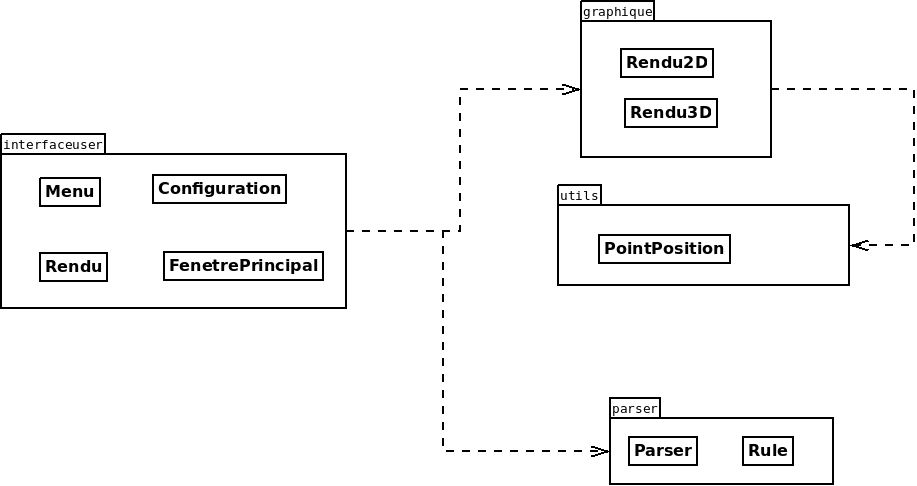
\includegraphics[width=16cm]{images/package.png}
	    \caption{Diagramme des packages }
\end{figure}
\begin{figure}[h]
		\centering
		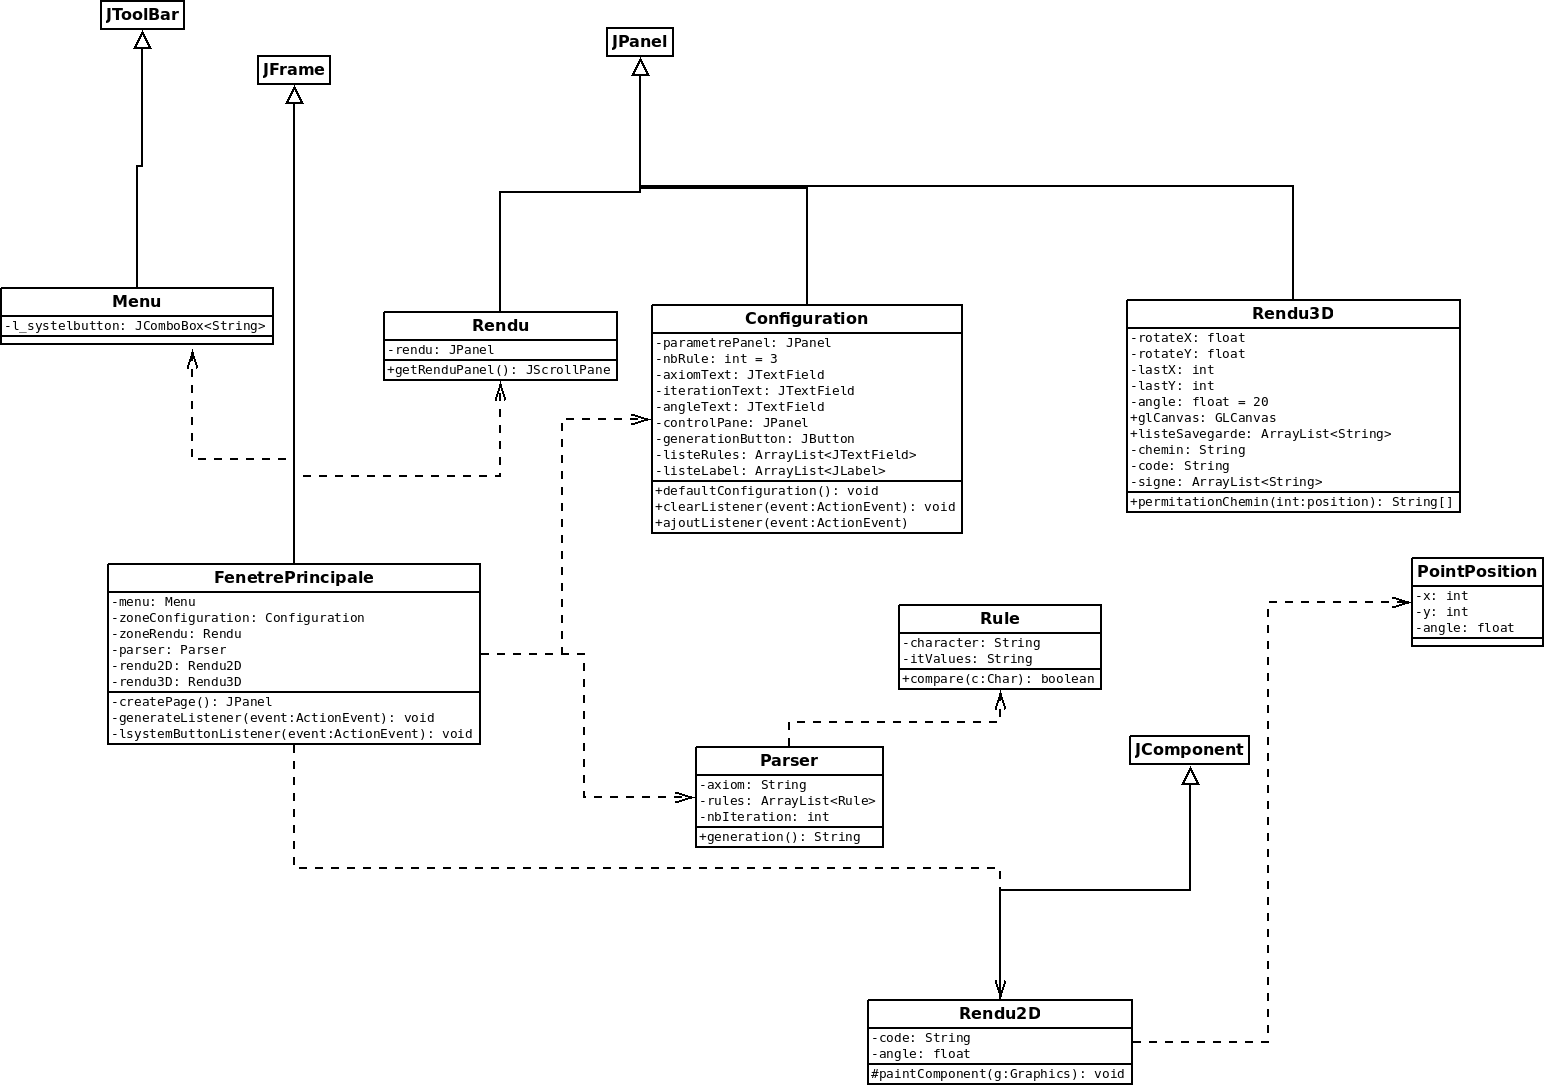
\includegraphics[width=18cm]{images/classe.png}
	    \caption{Diagramme des Classes }
\end{figure}
